\section{Anomalous Energy Loss Mechanisms\Contact{Maurizio}}
\Contributors{Maurizio, Oscar, (Alex), Zentner?, Sam McDermott}
\label{sec:cooling}


Observations of stars provide a mechanism to probe temperatures, particle densities, and time scales that are inaccessible to laboratory experiments.
Since conventional astrophysics allows us to quantitatively model the evolution of stars, the detailed study of stellar populations can provide a powerful technique to probe new physics.
In particular, if new light particles exist and are coupled to Standard Model fields, their emission would provide an additional channel for energy loss. 
Such anomalous energy loss mechanisms would change the time that stars spend in specific stellar evolutionary phases.
Such deviations are a robust predictions of light, weakly coupled particles, and the general agreement between observation and Standard Model predictions has been used to constrain the properties of many types of new particles \citep{hep-ph/0611350, 1210.1271, 1302.3884, 1305.2920, 1611.03864, 1611.05852, 1803.00993}.

While the predictions of the Standard Model are broadly consistent with observations of stellar evolution, several independent observations have shown a systematic preference for an additional subdominant energy-loss mechanism (see \citealt{Giannotti:2017hny} for a recent review).
These observations include red giants branch (RGB) stars, in particular the luminosity of the tip of the branch~\citep{Viaux:2013lha,Viaux:2013hca}; 
horizontal branch stars (HB), specifically by comparing the number of HB and RGB stars~\citep{Ayala:2014,Straniero:2015nvc};
variable white dwarf (WD) stars, for which the cooling efficiency was extracted from the rate of the period change~\citep{KeplerEtAl,Isern:1992gia,BischoffKim:2007ve,Corsico:2012ki,Corsico:2012sh,Corsico:2014mpa,Corsico:2016okh,Battich:2016htm}; 
and the WD luminosity function (WDLF), which describes the distribution of WDs as a function of their luminosity~\citep{Isern:2008nt,Bertolami:2014wua,Isern:2018uce}.
Observed discrepancies between these stellar measurements and predictions from conventional models of stellar cooling can be interpreted as the need for additional energy loss (\figref{axions}).
\cite{Giannotti:2015kwo} provide a systematic analysis of the new-physics interpretation of stellar observations  where cooling anomalies have been reported, and they conclude that axions and ALPs are the best candidates to account for the observed discrepancies. 
While these `hints' of anomalous cooling are subdominant deviations on broadly successful models of stellar evolution, it is imperative to explore possible signatures of new physics when they arise.

LSST will greatly improve our understanding of stellar evolution by providing unprecedented photometry, astrometry, and temporal sampling for a large sample of faint stars \citep{0912.0201}.
These observations will allow us to better assess the significance of claimed anomalies, and will further guide constraints on (or detection of) new physics.
A better understanding of astrophysical energy transport will ultimately help shed light on the physics of light, weakly-coupled particles and will offer an invaluable guide to future experimental searches for axions and ALPs~\citep{Irastorza:2018dyq}.

\begin{figure}[t]
\centering
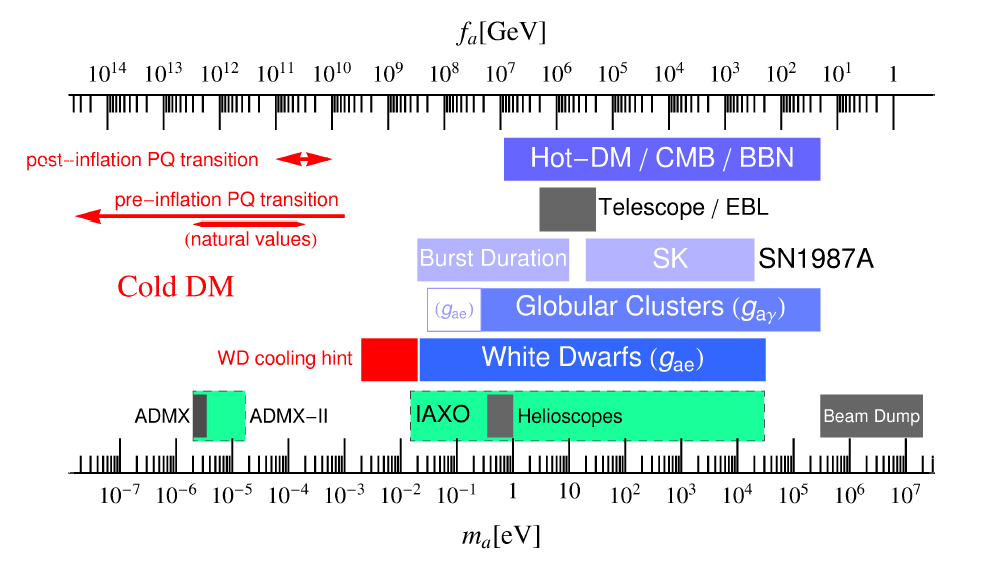
\includegraphics[width=0.6\columnwidth]{axions.png}
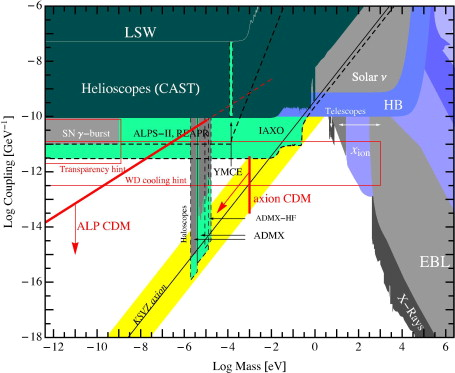
\includegraphics[width=0.39\columnwidth]{alps.jpg}
\caption{Left: Existing experimental and observational constraints on the QCD axion \citep{Redino:2015}.  
Right: Constraints on ALP coupling to photons \citep{Ringwald:2012}.
Astrophysical constraints and hints include observations of white dwarfs (WD), globular clusters (GC), supernova (SN), and horizontal branch stars (HB).
Note the wide range of mass and coupling scales that are constrained by these observations.
\label{fig:axions}
}
\end{figure}

\subsection{White Dwarf Luminosity Function}
\Contributors{Maurizio, Oscar, (Alex)}

The white dwarf luminosity function (WDLF) plays a particularly significant role in our understanding of stellar cooling and offers a fundamental method to test new physics.
Measurements of the slope of the WDLF can probe additional energy loss mechanisms and the production rate of the novel particle responsible for the nonstandard cooling.
The general agreement between the observed WDLF and predictions from standard astrophysics have been used to place bounds on the axion-electron coupling \citep{Isern:2008nt,Bertolami:2014wua}, on the anomalous neutrino magnetic moment \citep{Bertolami:2014noa}, on the kinematic coupling of dark photons to standard photons \citep{Chang:2016qfl}, and on the variation of the gravitational constant \citep{Althaus:2011ca}.
However, several recent analyses of the WDLF have shown a preference for additional energy loss with respect to the Standard Model predictions.
In particular, \cite{Bertolami:2014wua} used data from the Sloan Digital Sky Survey (SDSS) and the SuperCOSMOS Sky Survey (SCSS) to show a $2 \sigma$ discrepancy from the Standard Model prediction, which could be explained by axions coupling to electrons with $g_{\phi e}\simeq 1.4\times 10^{-13} \GeV^{-1}$.\footnote{The additional energy can also be accounted for by dark photons~\citep{Giannotti:2015kwo,Chang:2016qfl}, but not by anomalous neutrino electromagnetic form factors~\citep{Bertolami:2014noa}.}
These measurements of the WDLF have guided experimental searches for axions and ALPs, particularly the IAXO~\citep{Irastorza:2011gs,Armengaud:2014gea}, and ALPS II~\citep{Bahre:2013ywa,ALPSII} experiments.

Observations from the \Gaia satellite have already increased the catalog of WDs by an order of magnitude with respect to SDSS \citep{1805.01227,1807.03315,1807.02559}.
The growing sample of WDs with precisely measured distances will enable an improved measurement of the WDLF.  
However, the completeness of the \Gaia sample is limited to WDs within 100 pc~\citep{1807.03315}.
%Oscar. In the GAIA DR2 about 260.000 WDs have been identified. However the sample is complete up to G=20-21, only for those within 100 pc, which are about 11.000 stars. The major problem is that the completeness drops at low Galactic latitudes, and the magnitude limit of the catalogue varies significantly across the sky as a function of Gaia’s scanning law.  A larger and more complete sample will be certainly available with the final data release.
LSST is expected to detect WDs that are 5 to 6 magnitudes fainter than those detected by \Gaia, ultimately increasing the census of WDs to tens of millions~\citep{0912.0201}.
LSST will provide more complete and homogeneous samples of WDs, allowing for a significant reduction in both the statistical and systematic uncertainties in measurements of the WDLF. 
LSST is expected to measure hundreds of thousands of WDs in the Galactic halo, enabling the construction of reliable luminosity function of halo WDs. 
By deriving independent WDLFs from different Galactic populations it will be possible to reduce uncertainties related to star formation histories, and to ultimately provide a more clear assessment of the physical origin of the cooling anomalies \citep{Isern:2018uce}. 


\subsection{Globular Cluster Stars}
\Contributors{Maurizio, Oscar, (Alex)}


Massive stars, specifically those close to the helium burning phase, provide another excellent environment to study anomalous energy loss mechanisms. 
Generally, stellar evolutionary codes such as MESA \citep{1009.1622} provide a good model for the evolution of massive stars, allowing constraints to be placed on novel particle production \citep[\eg,][]{1210.1271,1611.05852}.
However, several recent analyses of giant branch stars have detected deviations from standard stellar models that can be interpreted as a signature of anomalous energy loss.
For example, studies have shown a brighter-than-expected tip of the RGB (TRGB) in the M5 globular cluster~\citep{Viaux:2013lha,Viaux:2013hca}, indicating somewhat over-efficient cooling during the evolutionary phase preceding the helium flash.
The anomalous brightness, $\Delta M_{I,{\rm TRGB}}\simeq 0.2$ mag in absolute $I$-band magnitude, observed in M5  can be interpreted as an anomalous cooling of a few $10^{33}$ erg/s.
Such cooling could be accounted for by a neutrino magnetic moment or an axion-electron coupling of the order of that predicted from the WDLF~\citep{Viaux:2013lha}. 
These constraints can be improved using multi-band photometry of multiple globular clusters \citep[\eg,][]{Straniero:2018fbv}.

Advances in the analysis of globular cluster RGB stars are currently limited by modeling uncertainties on the stellar evolution of the giant branch.
Fundamental improvements should be expected in the near future. 
In particular, exquisite astrometry from the {\it Gaia} satellite will precisely determine cluster distances, currently the largest sources of observational uncertainty in the determination of the absolute luminosity of the TRGB.\footnote{The {\it Gaia} data relevant for GCs are expected in 2022~\citep{Gaia}.}
Moreover, the angular resolution of the next-generation space-based missions, such as JWST~\citep{Gardner:2006ky}, will enlarge the statistical sample of RGB members near the cores of GCs. 
The brightness of RGB stars in nearby GCs limits the contributions of LSST, which saturates at $g \sim 17$ mag and suffers from crowding near the cores of GCs.
However, LSST will enable independent measurements of GC distances, providing a valuable handle on systematic uncertainties of {\it Gaia} observations.\footnote{The parallaxes of bright ($G<14$ mag) sources can be derived with a median uncertainty of 0.04 mas in {\it Gaia} DR2. However, for fainter stars the parallaxes become sensitive to systematic errors.  Presently, these systematics hamper a precise determination of GC distances \citep{Chen:2018}.}
Moreover, it is likely that the homogeneity of the LSST sample and the wide spectral range of LSST, will lead to an optimal calibration of the bolometric corrections for RGB and HB stars and ultimately contribute to a more clear assessment of the cooling of GC stars.


\subsection{Massive stars and core-collapse supernovae}
\Contributors{Oscar,Maurizio, (Alex), Sam McDermott}

The cores of massive stars are among the most powerful natural laboratories to investigate the possible production of weakly interacting light particles, particularly axions. 
The energy loss rate via axions is quite sensitive to temperature. 
For instance, the rate of the Primakoff process (the photon-axion conversion in the static electric field of ions and electrons) scales as $T^4$. 
Figure \ref{fig:massivestar} shows the evolution of the neutrino and axion luminosities in a $18\Msun$ stellar model. 
After He burning, the central temperature rapidly increases becoming larger than $10^9$ K. 
In standard stellar models (no axions or other non-standard cooling), the energy loss by neutrinos largely overcomes the energy loss by photons. Such an occurrence causes a rapid drop of the evolutionary time scale and determines the chemical and physical structure of the star at the onset of the core collapse. 
In this context, an additional energy loss induced by the possible production of axions may significantly affect the pre-explosive stellar structure and, in turn, may determine the final fate, namely, the success or failure of the supernova. 
Such an effect may be revealed by connecting core-collapse supernova to their massive star progenitors.

Another powerful strategy by which novel particles can be constrained is by considering the evolution of the neutrino cooling phase of nearby SN  \citep[\ie, SN1987A][]{Burrows:1988, Raffelt:1988}.
The simplest and most robust method by which such constraints can be implemented is the so-called ``Raffelt criterion'', which limits the luminosity of new particles to be below the luminosity of neutrinos during the neutrino-cooling phase \citep{hep-ph/0611350}.
Neutrino observations of SN1987A have been used to place limits on a wide variety of new particles \citep{hep-ph/0207098, 1611.03864, 1611.05852, 1803.00993, 1808.10136}.
Again, it is possible that a subdominant release of energy into new particles is responsible for resolving some lingering inconsistencies with the Standard-Model-only picture of core-collapse supernova explosion \citep{0806.4273, 1805.07381}, though such an effect is difficult to resolve analytically on top of other qualitative uncertainties of the Standard-Model-only picture \citep{1809.05106, 1811.11178}.
LSST, in combination with upcoming neutrino experiments (i.e., DUNE), will help reduce Standard Model uncertainties and expand this analysis to future and more distant SN \citep{1807.10334}.

\begin{figure}[t]
\centering
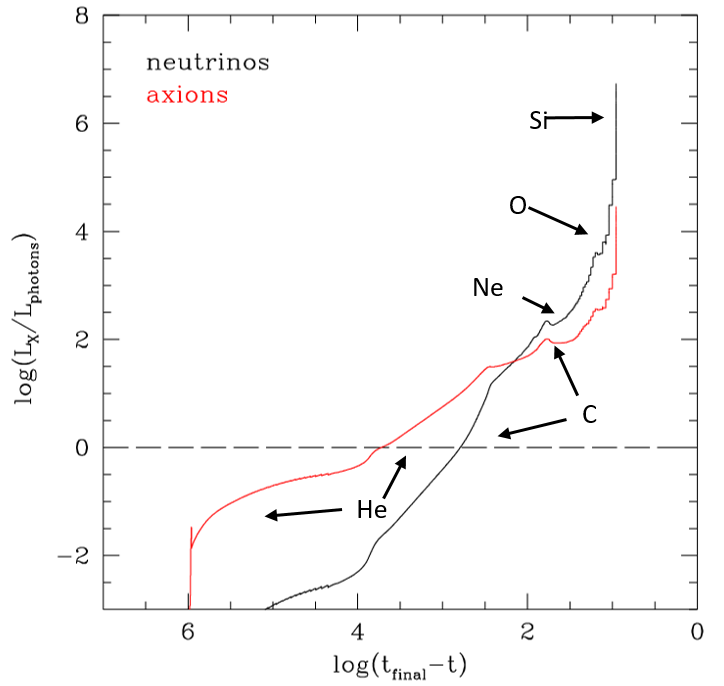
\includegraphics[width=0.5\columnwidth]{massivestar.png}
\caption{Evolution of the luminosties of neutrinos and axions, in a M=18 M$_\odot $ stellar model ($t$ in years), relative to the photon luminosity. The various evolutionary phases are indicated. 
%In the calculation of the axion rate we have assumed the presently available upper bounds, as obtained from astrophysical constraints, for the axion-photon and axion-electron coupling constants.
In the calculation of the axion rate, we have assumed the current upper bounds on the axion-photon and axion-electron coupling.
\ADW{Do we need a reference for this figure?}
}
\label{fig:massivestar}
\end{figure}

LSST is expected to discover $\roughly 3.5\times10^5$ core-collapse SNe per year \citet{Lien:2009}. \ADW{Better to update this from Goldstein et al. (2018).}
For most of these SNe, LSST will provide precise distances and, for a large sub-sample, it will be possible to identify their progenitors in pre-explosion images. \ADW{Is this true?}
So far, a clear identification of the progenitor star has been obtained only for about 20 type II SNe \citep{Smartt:2015}.  
The identification of a much larger number of massive stars before they explode is a mandatory step to understand the core-collapse SNe process and the possible activation of non-standard cooling processes during the late evolution of massive stars. 
Recent theoretical studies have investigated the conditions for which a massive star, after the core collapse, successfully bounces giving rise to a supernova \citep[e.g.,][and references therein]{OConnor:2011,Sukhbold:2016}.   
In particular, it was found that the ability to explode predominantly depends on the structure of the progenitor. 
%Therefore, the impact of LSST in this field is twofold: it will constrain the supernova engine and may provide hints for new physics beyond the standard model. 
Therefore, besides providing more clear insights in the supernova engine, LSST will provide a solid framework to test the presence of novel cooling channels efficient during pre-SN evolution, constraining or hinting at the existence of axions or other weakly interacting particles. 


%These observations indicate a systematic problem in our understanding of stellar cooling, showing in all cases the need for additional energy loss, as if an unknown cooling mechanism was at play. 
%Given the very different stars that exhibit the problem, it is not easy to provide a general mechanism to explain all the observations. 
%Among the new-physics options, axions and ALPs stand out as the best candidates to explain all the anomalous cooling observed~\citep{Giannotti:2015kwo}.
%However, the question remains ``are stars truly hinting at new-physics''? 
%Even though only dedicated axion experiments will be able to provide a definitive answer to this question, 

%
%The new-physics candidates that can account for the additional cooling are not limited to axions or ALPs. 
%Hidden photons could work too, for some range of mass and coupling~\cite{Giannotti:2015kwo,Chang:2016qfl}.
%
%The additional energy can also be accounted for by hidden photons~\cite{Giannotti:2015kwo} but not by anomalous neutrino electromagnetic form factors~\cite{Bertolami:2014noa}.
%Hidden photons could also explain the observations for specific mass and couplings~\cite{Giannotti:2015kwo}.

%Stars are powerful tools to probe new-physics, particularly the physics of light, weakly interacting particles such as axions and ALPs (\secref{axions}). 
%If these particles existed and were sufficiently strongly coupled to standard model fields, their emission would result in an excessive energy loss with respect to the standard model predictions.
%That would lead to changes in the time scales of specific evolutionary phases and could ultimately be traced from dedicated surveys of stellar populations.
%Intriguingly, a set of independent observations show a systematic preference for additional energy loss in many stellar systems (see \citealt{Giannotti:2017hny} for a recent review).
%These observations include red giants branch (RGB) stars, in particular the luminosity of the tip of the branch~\citep{Viaux:2013lha,Viaux:2013hca}; 
%horizontal branch stars (HB), specifically by comparing the number of HB and RGB stars~\citep{Ayala:2014,Straniero:2015nvc};
%variable white dwarf (WD) stars, for which the cooling efficiency was extracted from the rate of the period change~\citep{KeplerEtAl,Isern:1992gia,BischoffKim:2007ve,Corsico:2012ki,Corsico:2012sh,Corsico:2014mpa,Corsico:2016okh,Battich:2016htm};  
%and the WD luminosity function (WDLF), which describes the distribution of WDs as a function of their luminosity~\citep{Isern:2008nt,Bertolami:2014wua,Isern:2018uce}.

%Observed discrepancies between these stellar measurements and predictions from conventional models of stellar cooling can be interpreted as the need for additional energy loss.
%These observations indicate a systematic problem in our understanding of stellar cooling, showing in all cases the need for additional energy loss, as if an unknown cooling mechanism was at play. 
%Given the very different stars that exhibit the problem, it is not easy to provide a general mechanism to explain all the observations. 
%\cite{Giannotti:2015kwo} provided a systematic analysis of the new-physics interpretation of all stellar systems where cooling anomalies have been reported, and they concluded that axions and ALPs are the best candidates to account for the observed discrepancies. 
%Among the new-physics options, axions and ALPs stand out as the best candidates to explain all the anomalous cooling observed~\citep{Giannotti:2015kwo}.
%However, the question remains ``are stars truly hinting at new-physics''? 
%Even though only dedicated axion experiments will be able to provide a definitive answer to this question, 
%LSST will provide a much larger sample of faint stars with improved photometry allowing us to asses the observational significance of these anomalies and further guide solutions involving new-physics.
%This will ultimately shed light on the physics of axions and offer an invaluable guide to the future experimental searches for axions and ALPs~\citep{Irastorza:2018dyq}.

% GC section
%A complete understanding of the cooling during RGB evolution, and in particular an assessment of the possibility that a novel cooling mechanism is at play, requires more statistics.
%$ g_{ae} \sim (1 - 2) \times 10^{-13}$ .
%
%An independent way of testing the physics of stellar cooling is to compare stellar populations in different evolutionary stages. 
%The most common option is to measure the  R-parameter, $R= {N_{\rm HB}}/{N_{\rm RGB}}$, which compares the numbers of stars in the horizontal branch (HB) and in the upper portion of the RGB.
%This technique has been often adopted in the past to provide a bound on the axion coupling to photons~\citep{Raffelt:1985nk,Raffelt:1987yu}.
%More recent analyses~\citep{Ayala:2014,Straniero:2015nvc} showed a disagreement (at the $2\sigma$-level) between the observed and expected value of $R$.
%More specifically, the R-parameter derived from observations was found to be smaller than expected, indicating a surplus of RGB with respect to HB stars in the examined clusters.
%This suggests that HB stars are cooling more efficiently (and are, therefore, less numerous) than expected, a result that may be interpreted in terms of an ALP coupled to photons with $ g_{\phi\gamma}=(0.29-0.57)\times 10^{-10} {\rm GeV}^{-1}$~\citep{Straniero:2015nvc}.
%
%, which could be interpreted as due to new-physics. 
%%Specifically, the observed $ R=1.39\pm 0.03 $ is smaller than the expected one $ 1.44\leq R\leq 1.50$. 
%
%As in the case of the WDLF, the results from giant branch stars are far from definitive. The significance of the observed discrepancies is still low and more statistics are required to reliably assess these anomalies.  


%Finally, LSST will contribute novel observations of RGB stars throughout the Local Volume.  It will be sensitive to RGB stars 1.5 mag below the TRGB in Local Volume galaxies out to $\roughly6\Mpc$ \citep{0912.0201}.
%In regions of high surface brightness, the resolution limit of LSST will reduce the accessible volume. 
%However, for surface brightnesses of $\mu \sim 27$ mag/arcsec$^2$, LSST is still expected to reach 1 mag below the TRGB for galaxies out to 4\Mpc.
%Dwarf galaxies contain significantly more RGB stars than GCs but are considerably more complex and less homogeneous. 
%Thus, while these observations should greatly enhance our understanding of the stellar evolution on the RGB, it is not yet clear how much they will contribute to our understanding of stellar cooling anomalies. 

%Ultimately, these extra-galactic observations may not add much insight to  what one can learn from the analysis of galactic GCs, although only the data analysis will 
%Studying such extra-galactic stars is, however, a fascinating new possibility (prohibited with the current telescopes) to investigate in the near future. 

%By providing deep, homogeneous photometry for billions of stars in the Milky Way and Local Group, LSST will enable major advances in our understanding of stellar populations. The larger statistics and reduced uncertainty in the globular cluster distances, currently the largest sources of observational errors in the determination of the absolute luminosity of the TRGB, will greatly improve the confidence we have in these results.\footnote{Results from the Gaia mission will also reduce significantly the uncertainties in the stellar distances. The data relevant for globular clusters is expected for 2022~\citep{Gaia}.}

%Particularly important will be the reduced uncertainties in the Globular Cluster distances, currently the largest sources of observational errors, expected from LSST and from the GAIA mission~\cite{Gaia}. 

%Oscar: Till now, the GAIA collaboration encountered some problems with GC parallaxes (at least with the DR2). Maybe LSST could improve GC distances.      

%Coupling between axions and standard model particles can provide an additional energy loss mechanism that could be detected through observations of hot, dense environments.  Specifically, the cooling rate of white dwarf stars provides an important avenue towards constraining additional energy loss mechanisms. In particular, \citet{0806.2807} claim a hint of anomalous cooling in the white dwarf luminosity function measured by SDSS. Inclusion of axion cooling improves the agreement between the theoretical predictions and observation  The best fit is obtained for $m_a \cos^2 \beta \sim 5 \text{meV}$, where $m_a$ is the mass of the axion and $cos^2 \beta$ is a free parameter. The wide area survey of LSST will increase measurements of the white dwarf luminosity function by several magnitudes increasing the census of white dwarfs from tens of thousands with SDSS to tens of millions with LSST \citep{0912.0201}. In addition, LSST photometry will be $\roughly 3$ times as accurate as SDSS. Together, this improved data set will significantly decrease both the statistical and systematic uncertainties on modeling the WDLF.
